\section{Bestehende Sensornetze} % wie FS 20 und HM
\myContentSectionFrame[\thesection - 6]

\againframe{netzwerkaufbau}
%-------------------------------------------------------------------------------

\begin{frame}{\insertsubsection}{Interessante Fragestellungen}
	\begin{itemize}
	\item 	Ist es möglich, bestehende Sensornetztechnologien in unseren Ansatz zu integrieren?
	\item 	Welche Vor- und Nachteile bietet die Integration solcher Technologien?
	\item 	Was bringt der Einsatz von CoAP zum Ansprechen der Fremdkomponenten?
	\end{itemize}
	\vspace{0.5em}
	\begin{center}
		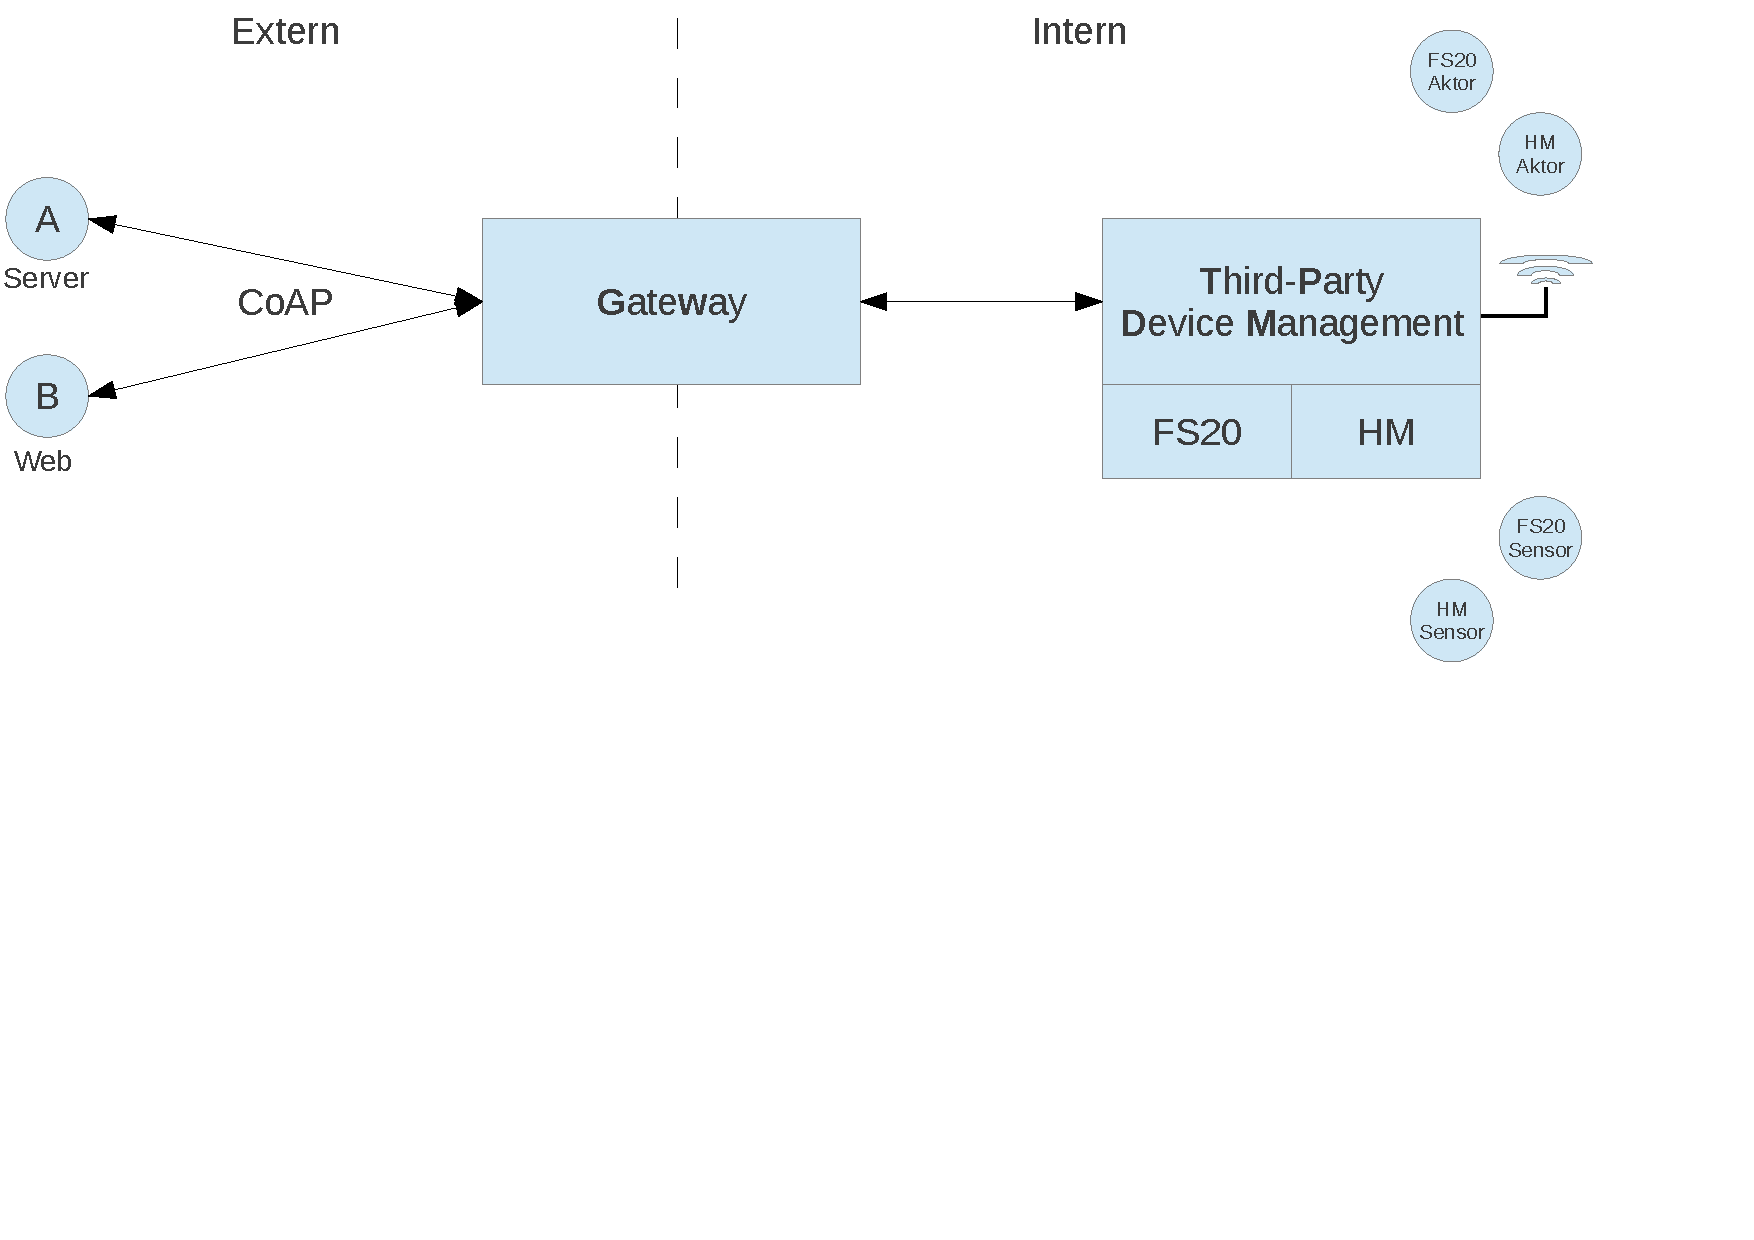
\includegraphics[scale=0.38]{pic/gateway_ueberblick}
	\end{center}
\end{frame}

%-------------------------------------------------------------------------------

\begin{frame}{Gateway in bestehenden Sensornetzen}{Lösungsansätze HomeMatic/FS20}
	\begin{itemize}
	\item 	Reverse-Engineering
		\begin{itemize}
		\item 	Mitlesen von Nachrichten
		\item 	Analyse des HomeMatic-Protokolls
		\item 	Heranziehen alternativer Informationsquellen
		\end{itemize}
	\item Erkenntnisse in Programm umsetzen
		unter Berücksichtigung der Anbindung zum Gateway
\end{itemize}
\end{frame}


%-------------------------------------------------------------------------------

\begin{frame}{\insertsubsection}{Ergebnisse I}
	\begin{itemize}
	\item 	Integration von bestehenden Sensornetztechnologien ist möglich, aber aufwendig
	\end{itemize}
	\vspace{1em}
	Nutzung von bestehenden Sensornetzen:
	\begin{proconlist}
	\pro 	Reduzierung Entwicklungsaufwand der Hardware
	\pro 	Vorteile des jeweiligen Systems nutzbar
	\pro 	Systemübergreifender Einsatz
	\contra Verzicht auf Funktionalität
	\contra hoher Aufwand bei geschlossenen Systemen
	\end{proconlist}
\end{frame}

%-------------------------------------------------------------------------------

\begin{frame}{\insertsubsection}{Ergebnisse II}
	\begin{itemize}
	\item 	Gateway (CoAP $ \leftrightarrow $ bestehende Sensornetze)
	\end{itemize}
	\vspace{1em}
	\begin{proconlist}
	\pro 	standardisierte Schnittstelle für den Zugriff auf die Fremdkomponenten
	\contra für jedes System und Geräteklasse ist Ressource (PUT/GET) zu implementieren
	\end{proconlist}
\end{frame}
